
\section{The Charge Distribution of the H\protect\( _{2}\protect \)O Molecule}

Name \rule{2.0in}{0.1pt}\hfill{}Section \rule{1.0in}{0.1pt}\hfill{}Date
\rule{1.0in}{0.1pt}

\textbf{Introduction}

In this exercise you will make a theoretical investigation of the
charge distribution within a water molecule (H\( _{2} \)O). The molecule
is electrically neutral and is made of 10 positive electric charges
and 10 negative electric charges (8 protons and electrons from the
oxygen atom and 1 proton and electron from each of the two hydrogen
atoms). Despite the net electrical neutrality of the molecule it can
produce an electric field if the positive and negative charges within
it have different configurations. If the most probable position of
the positive charges in the molecule does not coincide with the most
probable position of the negative charges as shown in Figure 1a, then
we call that configuration an electric dipole. Another candidate for
the charge distribution of H\( _{2} \)O is shown in Figure 1b and
is called an electric quadrupole. The most probable position of the
positive charge is either above or below the x-axis while the negative
charge is most likely to be found at the origin. This 'probabilistic'
view of the location of the charges is the basis of quantum mechanics,
the theory describing the subatomic world. Below you will calculate
the electric potential for these two charge distributions and you
will use your results to find the electric field for the dipole and
quadrupole. You will then consider the design of an experiment to
distinguish between the two different charge distributions.

\vspace{0.3cm}
{\centering 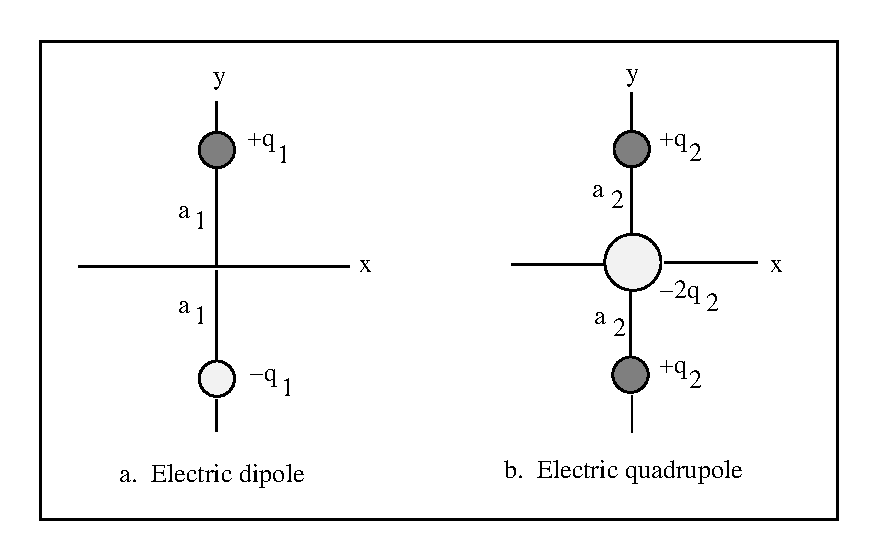
\includegraphics{charge_dist_water_mol/charge_dist_water_mol_fig_1.eps} \par}
\vspace{0.3cm}

\textbf{Activity 1: The Electric Dipole }

(a) Calculate the electric potential, \( V \), for the electric dipole for
a point along the y-axis, but at a position \( \left| y\right|  \)>
a\( _{1} \). Your final expression should depend on the position,
\( y \), the charge, q\( _{1} \), and the most probable location of the
charges, a\( _{1} \).
\vspace{40mm}

(b) Generate an expression for the potential energy, \( U \), of the charge
distribution when another charge, $q_{test}$,  placed somewhere
on the y-axis with \( \left| y\right|  \)> a\( _{1} \).
\vspace{40mm}

(c) Recall the component of the force on a particle is related to
the potential energy of the particle by F\( _{y} \) = -\( \frac{dU}{dy} \).
Calculate the force on the test charge in terms of the position on
the y-axis, the charges, and a\( _{1} \).
\vspace{40mm}

(d) Make the approximation that the test charge is far from the molecule,
i.e., \( \left| y\right|  \) \( \gg  \) a\( _{1} \), to generate
a new expression for the force.
\vspace{40mm}

\textbf{Activity 2: The Electric Quadrupole} 

(a) Calculate the electric potential, \( V \), for the electric quadrupole
for a point along the y-axis, but at a position \( \left| y\right|  \)
> a\( _{2} \). Your final expression should depend on the position,
\( y \), the charge, q\( _{2} \), and the most probable location of the
charges, a\( _{2} \).
\vspace{40mm}

(b) Generate an expression for the potential energy, \( U \), of the charge
distribution when another charge, $q_{test}$, is placed somewhere
on the y-axis with \( \left| y\right|  \) > a\( _{2} \).
\vspace{40mm}

(c) Calculate the force on the test charge in terms of the position
on the y-axis, the charges, and a\( _{2} \).
\vspace{40mm}

(d) Make the approximation that the test charge is far from the molecule,
i.e., \( \left| y\right|  \) \( \gg  \) a\( _{2} \), to generate
a new expression for the force.
\vspace{40mm}

\textbf{Activity 3: Distinguishing Between the Two Different Charge
Distributions} 

(a) Construct a table in the space below with column headings \( y \)(angstroms),
Dipole Force (arbitrary units), and Quadrupole Force (arbitrary units).
The units of distance known as angstroms are commonly used in atomic
physics. One angstrom is equal to 10\( ^{-10} \) m.
\vspace{40mm}

(b) To calculate the force on the test charge one must know the charges
and their positions for each charge distribution (q\( _{1} \), q\( _{2} \),
a\( _{1} \), a\( _{2} \)). These quantities are unknown to us at
this point. However, we want to compare the behavior of the force
due to each as a possible probe of the molecule's charge distribution.
In the expressions you generated in step (d) of Activities 1 and 2
for \( \left| y\right|  \) \( \gg  \) a\( _{1} \) or \( \left| y\right|  \)
\( \gg  \) a\( _{2} \) the forces depend on some power of \( y \). For
\emph{convenience}, set the constant in front of this power of \( y \) to
unity. Calculate the forces for the dipole and quadrupole at distances
between 1.5 angstroms and 5.0 angstroms in 0.5 angstrom steps. Enter
your results in the table.

(c) Make a graph of the force due to the dipole and due to the quadrupole
as a function of \( y \). Insert a copy of the graph into your notebook.

(d) In many experiments constants like those in your expressions for
the force on the test charge are unknown or poorly known. Suppose,
however, that you are able to accurately measure the radial dependence
of the force on $q_{test}$ at distances far from the H\( _{2} \)O
molecule. If that is the case use the results from steps (b) and (c)
to propose a technique to distinguish between the two candidates for
the charge distribution of H\( _{2} \)O. Support your proposal with
a mathematical argument. (Hint: Consider a ratio involving the measured
force.)
\vspace{40mm}

(e) Experiment has found that water behaves as an electric dipole
with the electric dipole moment, q\( _{1} \)a\( _{1} \), measured
to be 6.2 x 10\( ^{-30} \) C-m. If the charge that creates the dipole,
q\( _{1} \), is the charge associated with the protons and electrons
of the molecule calculate the separation of the charges, a\( _{1} \).
How does it compare with the size of the H\( _{2} \)O molecule of
about 1.0 angstroms?\vspace{40mm}

